\section{Graphics Processing Units}
Dedicated Graphic Processing Units (``GPUs'') are very common in desktop and laptops. \citep{STEAMHW}
GPUs are commonly used in the private and professional world, for computer gaming and accelerating graphic intensive programs such as Adobe Photoshop and 3D modelling tools. \citep{NVIDIAADOBE}
Their architecture can also be used for advantageously for certain types of computations, primarily computations which can be done in parallel. 
An example of this can be calculating different properties of the pixels on a screen. 
The screen can then be divided into different sections and the computations for each section is divided over the GPU.
This is possible because the calculations do not require results from the other calculations.
The same can be said of matrices used in mathematics.
The before mentioned example can be viewed as a matrix being divided into sections, so the same method of parallelised workflow can be used when multiplying two matrices.

\begin{figure}[h!]
\centering
 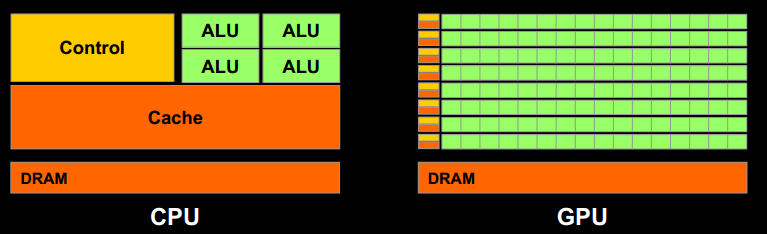
\includegraphics[width=1\textwidth]{figures/GPUCPUimage.png} % trim=4.85cm 15cm 0.85cm 1cm
\caption{A basic representation of the Transistor allocation on a GPU compared to a CPU}\label{image:GPUCPUimage} %ftp://download.nvidia.com/developer/cuda/seminar/TDCI_Arch.pdf
\vspace{-15pt}
\end{figure}

A simple representational comparison of a Central Processing Unit's (``CPU'') and a GPU's transistor usage is shown in \myref{image:GPUCPUimage}.
In the GPU there are many less powerful cores, however the total computation capacity is higher. 
As of Q1 2015 an example of a modern high end desktop CPU is the Intel Haswell core i7 5960X which has a theoretical peak of 384 giga- floating operations pr. second (GFLOPS) over 8 cores. \citep{puget}
A contemporary high end GPU is the NVIDIA GTX 980 which has 4616 GFLOPS, for single precision with 2048 CUDA cores. \citep{techpowerup,gtx980}
This results in the GPU being able to perform about 12 times more FLOPS compared to the CPU, meaning that it can process more data. 

This makes GPU an obvious target for computation, even some which are not graphical. % Antagende/konkluderende?!?